\documentclass{article}
\usepackage{arxiv}

\usepackage[utf8]{inputenc}
\usepackage[english, russian]{babel}
\usepackage[T1]{fontenc}
\usepackage{url}
\usepackage{booktabs}
\usepackage{amsfonts}
\usepackage{nicefrac}
\usepackage{microtype}
\usepackage{lipsum}
\usepackage{graphicx}
\usepackage{natbib}
\usepackage{doi}
\usepackage{amsmath}
\usepackage{bbm}  % для \mathbbm{1}
\usepackage{dsfont}  % для \mathds{1}





\title{Нейросетевые подходы к решению задачи оттока абонентов}

\author{ Батарин Егор Владиславович \\
	Кафедра алгоритмов и технологий программирования \\
	Московский физико-технический институт\\
	Москва \\
	\texttt{batarin.ev@phystech.edu} \\
	%% examples of more authors
	\And
	Джумакаев Тимур Казбекович \\
	Мегафон\\
	Москва\\
}
\date{}

\renewcommand{\shorttitle}{\textit{arXiv} Template}

%%% Add PDF metadata to help others organize their library
%%% Once the PDF is generated, you can check the metadata with
%%% $ pdfinfo template.pdf
\hypersetup{
pdftitle={Нейросетевые подходы к решению задачи оттока абонентов},
pdfsubject={q-bio.NC, q-bio.QM},
pdfauthor={Батарин Егор Владиславович, Джумакаев Тимур Казбекович},
pdfkeywords={CatBoost, Модель Кокса, Анализ выживаемости, Dynamic DeepHit},
}

\begin{document}
\maketitle

\begin{abstract}

В работе решается задача прогнозирования оттока абонентов компании Мегафон. Задача рассматривается как многоклассовая классификация, где в качестве меток класса выбраны факты оттока в будущие месяцы и факт отсутствия оттока в эти месяцы. Предлагаются различные подходы к решению задачи, как классические подходы: градиентный бустинг и модель Кокса, так и более современные подходы, связанные с применением методов глубокого обучения в моделях выживаемости. Проводится сравнение различных подходов с точки зрения принятых в работе критериев качества. В роли критериев качества модели выступают метрики Precision, Recall, F1, вычисленные при различных вероятностных порогах - числах, позволяющих перевести вероятности классов в метки классов. Цель работы заключается в поиске новых подходов к решению задачи оттока, которые покажут более высокие результаты по выбранным критериям качества, чем у текущих бейзлайнов. Эксперименты проведены на внутренних абонентских данных Мегафона.   

\end{abstract}


\keywords{CatBoost \and Модель Кокса \and Анализ выживаемости \and DeepHit  \and Dynamic DeepHit}

\section{Введение}

Данная работа посвящена решению задачи прогнозирования оттока в контексте телекоммуникационной отрасли в рамках проекта компании Мегафон. Данная задача позникает в большом количестве различных индустрий и для ее решения используются разные подходы. \cite{Ahn2020}. Среди всех таких подходов, включающих в себя разные современные методы машинного обучения (SVM, Random Forest, Gradient Boosting) основным направлением исследований для решения данной задачи был выбран анализ выживаемости. 

Классической работой по анализу выживаемости является модель пропорциональных рисков \cite{Cox1972}. В настоящее время появилось много новых подходов, так или иначе задействующих глубокое обучение \cite{Wiegrebe2024}. Эти подходы расширяют классические модели анализа выживаемости, позволяя обойти некоторые предположения о данных, которые на практике редко выполняются, например, предположение о пропорциональности рисков. Все модели анализа выживаемости можно разделить на две категории с зависимости от того, считается ли время непрерывным или дискретным. Поскольку специфика проекта Мегафона требует рассмотрения дискретного времени, то именно такой случай фигурирует в постановке задачи. 

Одной из известных дискретных моделей выживаемости является модель DeepHit \cite{Lee2018}, а также ее развитие - модель Dynamic DeepHit \cite{Lee2020}. В архитектурах обеих моделей используются нейросети, причем во второй модели помимо многослойного перцептрона применяется рекуррентная нейросеть RNN, а также механизм внимания. Данные работы взяты за основу для исследования в данной работе, их оригинальные версии и модицикации сравниваются для выявления лучшей модели.

Одним из самых распространенных подходов к задаче является градиентый бустинг \cite{Ahmad2019}.  В данной работе в качестве базового подхода рассматривается категориальный бустинг от компании Яндекс \cite{Dorogush2018}. Он получил большое распространение на российском рынке, поэтому исследуемые в работе подходы, основанные на анализе выживаемости, сравниваются с CatBoost.

В работе используются внутренние датасеты компании Мегафон, собранные на основе данных в КХД. В роли критериев качества модели выступают метрики Precision, Recall, F1, вычисленные при различных вероятностных порогах - числах, позволяющих перевести вероятности классов в метки классов.
\section{Постановка задачи}

\subsection{Общая постановка задачи анализа выживаемости}

В дискретном случае время имеет вид $\mathcal{T}=\{0,\ldots,T_{\max}\}$, где $T_{\max}$ - это максимальный горизонт предсказания (например, максимально возможное время жизни абонента). В любой их этих моментов может произойти событие $\mathcal{K}=\{\emptyset,1,\cdots,K\}$, где все события $\{1,\cdots,K\}$ соответствуют факту оттока по одной из $K$ возможных причин в некоторый момент времени $\tau$, а событие $\emptyset$ означает факт правого цензурирования - информация о том, что отток произойдет не раньше того времени $\tau$, когда произошло цензурирование, но точно неизвестно когда именно. Для каждого момента времени, таким образом, мы можем написать $\tau^i=\min(T^i,C^i)$, где $T^{i}\in\mathcal{T}$ - это времена наступлений одного из событий $\{1,\cdots,K\}$, а $C^{i}\in\mathcal{T}$ соответствует право-цензурированным событиям $\emptyset$. Имея в распоряжении информацию о произошедших событиях (включая цензурирования) $\{\tau^{i},k^{i})\}_{i=1}^{N}$ и некоторую дополнительную информацию о признаках абонентов, мы хотим научиться предсказывать вероятности наступления события из $\mathcal{K}$ в будущем. В зависимости от того, рассматриваем ли мы признаки абонентов только в один момент времени (как в случае модели DeepHit) или рассматриваем для каждого абонента временной ряд соотвествующих ему признаков (как в случае модели Dynamic DeepHit), будет немного различаться математическая постановка задачи. 

Специфичным для анализа выживаемости критерием качества является C-индекс (concordante index) \cite{Alabdallah2022}, являющийся аналогом широкого известного критерия качества AUC. Он численно равен доле пар абонентов, которые модель верно упорядочила с точки зрения функции выживаемости. Пара $(i,j)$, где $\tau_i < \tau_j$ - моменты наступлений события оттока $k$, считается верно упорядоченной, если для оцененных моделью условных функций выживания $\hat{F}_{k,i}$ и $\hat{F}_{k,j}$ при условии наступления признаков $i$ и $j$ соответственно, выполнено неравенство: 

$$ \hat{F}_{k,i}(\tau_i ) >  \hat{F}_{k,j}(\tau_i ) $$ 

Этот индекс отражает то разумное требование к моделям выживаемости, которое заключается в том, что для абонентов, которые оттекают рано, оценочная условная функция распределения должна возрастать быстрее, так как для них целевое событие наступило при меньших значениях времени. 

\subsection{Модель DeepHit}

В данной модели предполагается, что абонент полностью описывается вектором $\bold{x} \in X$, соответственно обучающая выборка имеет вид $\mathcal{D}=\{(\mathbf{x}^{(i)},\tau^{(i)},k^{(i)})\}_{i=1}^N$, вероятности нецензурированных событий $k^* \neq \emptyset $ имеют вид $P(\tau=\tau^*,k=k^*|\mathbf{x}=\mathbf{x}^*)$, а функция распределения имеет вид:

\begin{align}
	F_{k^*}(t^*|\mathbf{x}^*) &= P(\tau\leq t^*,k=k^*|\mathbf{x}=\mathbf{x}^*) 
	= \sum_{\tau^*=0}^{t^*} P(\tau=\tau^*,k=k^*|\mathbf{x}=\mathbf{x}^*).
\end{align}

Поскольку теоретическая функция распределения неизвестна, то рассматривается ее оценка 
\begin{equation}
	\begin{aligned}
\hat{F}_{k^*}(\tau^*|\mathbf{x}^*)=\sum_{m=0}^{\tau^*}o_{k,m}^*
	\end{aligned}
\end{equation}

 на основе ответов модели DeepHit: $\mathbf{o}=[o_{1,1},\cdots,o_{1,T_{\max}},\cdots,o_{K,1},\cdots,o_{K,T_{\max}}]$, где $o_{k,\tau}$ - оценка моделью DeepHit вероятности того, что событие оттока $k$ произойдет в момент времени $\tau$.

В качестве функции потерь используется сумма двух слагаемых $\mathcal{L}_{\mathrm{Total}}=\mathcal{L}_1+\mathcal{L}_2$, в которой первое слагаемое имеет вид: 
\begin{equation}
	\begin{aligned}
		\mathcal{L}_{1} & = -\sum_{i=1}^N \left[\mathbbm{1}(k^{(i)}\neq\emptyset)\cdot\log\left(y_{k^{(i)},\tau^{(i)}}^{(i)}\right)  + \mathbbm{1}(k^{(i)}=\emptyset)\cdot\log\left(1-\sum_{k=1}^K\hat{F}_k(\tau^{(i)}|\mathbf{x}^{(i)})\right)\right]
	\end{aligned}
\end{equation}

и оно отвечает за логарифмическое правдоподобие, а второе слагаемое имеет вид: 
\begin{equation}
	\begin{aligned}
\mathcal{L}_2=\sum_{k=1}^K\alpha_k\cdot\sum_{i\neq j}A_{k,i,j}\cdot\eta\left(\hat{F}_k(\tau^{(i)}|\mathbf{x}^{(i)}),\hat{F}_k(\tau^{(i)}|\mathbf{x}^{(j)})\right)
	\end{aligned}
\end{equation}

где $A_{k,i,j} = \mathbb{I}(k^{(i)}=k,\tau^{(i)}<\tau^{(j)})$ - индикатор того, что событие $k$ наступает для $j$-ого абонента позже, чем для $i$-ого и функция
$\eta(x,y)=\exp\left(\frac{-(x-y)}{\sigma}\right)$. Эта добавка тем меньше, чем лучше модель упорядочивает абонентов с точки зрения C-индекса. 



\subsection{Модель Dynamic DeepHit}

Эта модель является расширением предыдущей и для каждого абонента $i$ в ней рассматривается уже не единственный вектор-признак $\bold{x}_i$, а временной ряд векторов-признаков: 
$$\mathcal{X}^i(t)=\{\mathbf{x}^i(t_j^i):0\leq t_j^i\leq t\mathrm{~for~}j=1,\cdots,J^i\}$$, где $\mathbf{x}^i(t_j)$ - это вектор признак $i$-ого абонента, замеренный в момент времени $t_j$ и равный $\mathbf{x}_j^i=[x_{j,1}^{i},\cdots,x_{j,d_{r}}^{i}]$. Кроме того, в этой модели для каждого абонента $i$ вводится набор векторов-флагов $\mathrm{M}^i=\{\mathrm{m}_1^i,\cdots,\mathrm{m}_{J^i}^i\}$, $\mathbf{m}_j^i=[m_{j,1}^i,\cdots,m_{j,d_x}^i]$, которые сигнализируют о пропущенных значениях: $m_{j,d}^{i}=1$ тогда и только тогда, когда $x_{j,d}^{i}$ пропущено, иначе $m_{j,d}^{i}=0$. Напоследок, вводится последовательность векторов временных интервалов между замерами времени $\Delta_i = \{\delta_{1}^{i},\delta_{2}^{i}\cdots,\delta_{J^{i}}^{i}\}$, где $\delta_{j}^{i}=t_{j+1}^{i}-t_{j}^{i}$ для всех $1\leq j<J^{i}$ и $\delta_{J^i}^i=0$. В итоге получается обучающая выборка: $\mathcal{D}=\{(\mathbf{X}^{i},\mathbf{M}^{i},\Delta^{i},\tau^{i},k^{i})\}_{i=1}^{N}$.

Теоретическая функция распределения в модели Dynamic DeepHit принимает вид:

\begin{equation}
	\begin{aligned}
		F_{k^{*}}(\tau^{*}|\mathcal{X}^{*}) & = P(T\leq\tau^{*},k=k^{*}|\mathcal{X}^{*},T>t_{J^{*}}^{*}) = \\
		& =\sum_{\tau\leq\tau^*}P(T=\tau,k=k^*|\mathcal{X}^*,T>t_{J^*}^*).
	\end{aligned}
\end{equation}

Теоретическая функция выживания вычисляется следующим образом:

\begin{equation}
	\begin{aligned}
		S(\tau^{*}|\mathcal{X}^{*}) & = 
		 	P(T>\tau^*|\mathcal{X}^*,T>t_{J^*}^*) =\\
		& =1-\sum_{k\neq\emptyset}F_k(\tau^*|\mathcal{X}^*)
	\end{aligned}
\end{equation}

Поскольку теоретические функции неизвестны, мы можем пользоваться только оценочными. Оценочная функция распределения выражается через ответы модели Dynamic DeepHit:
\begin{equation}
	\begin{aligned}
\hat{F}_{k^*}(\tau^*|\mathcal{X}^*)=\frac{\sum_{t_{J^*}^*<\tau\leq\tau^*}o_{k^*,\tau}^*}{1-\sum_{k\neq\emptyset}\sum_{n\leq t_{J^*}^*}o_{k,n}^*}
	\end{aligned}
\end{equation}

Функция потерь состоит из трех частей: $\mathcal{L}_{\mathrm{Total}}=\mathcal{L}_1+\mathcal{L}_2+\mathcal{L}_3$. Слагаемые $\mathcal{L}_1$ и $\mathcal{L}_2$ аналогичны соответствующим слагаемым из модели DeepHit и имеют вид: 

\begin{equation}
	\begin{aligned}
		\mathcal{L}_{1} & =-\sum_{i=1}^N\left[\mathbbm{1}(k^i\neq\emptyset)\cdot\log\Big(\frac{o_{k^i,\tau^i}^i}{1-\sum_{k\neq\emptyset}\sum_{n\leq t_{Ji}^i}o_{k,n}^i}\Big)\right] \\
		& +\mathbbm{1}(k^i=\emptyset)\cdot\log\biggl(1-\sum_{k\neq\emptyset}\hat{F}_k(\tau^i|\mathcal{X}^i)\biggr)\biggr]
	\end{aligned}
\end{equation}

\begin{equation}
	\begin{aligned}
\mathcal{L}_2=\sum_{k=1}^K\alpha_k\sum_{i\neq j}A_{kij}\cdot\eta\left(\hat{F}_k(s^i+t_{J^i}^i|\mathcal{X}^i),\hat{F}_k(s^i+t_{J^j}^j|\mathcal{X}^j)\right)
	\end{aligned}
\end{equation}
, где $s^i=\tau^i-t_{J^i}^i$, $A_{kij}=\mathbbm{1}(k^i=k,s^i<s^j)$ , $\eta(a,b)=\exp\left(-\frac{a-b}{\sigma}\right)$


Третье слагаемое в общей функции потерь является новым и отвечает за регуляризацию временных рядов: 

\begin{equation}
	\begin{aligned}
	\mathcal{L}_3=\beta\cdot\sum_{i=1}^N\sum_{j=0}^{J^i-1}\sum_{d\in\mathcal{I}}(1-m_{j+1,d}^i)\cdot\zeta(x_{j+1,d}^i,y_{j,d}^i)	
	\end{aligned}
\end{equation}		

Здесь $\mathcal{I}$ определяет подмножество зависящих от времени признаков абонентов, по которым мы хотим провести регуляризацию. 

\section{Численные эксперименты}


\subsection{Описание данных}

Эксперименты проводились на данных компании Мегафон, собранных с начала апреля 2024 до конца октября 2024. 

Обучающая выборка состоит из 2.7 миллионов примеров, валидационная и тестовая выборки содержат по 600 и 800 тыс. обучающих примеров соответственно. 

Для модели DeepHit обучающая выборка предварительно была нормирована. Для CatBoost нормировка не проводилась.

\subsection{Критерии качества}

Для анализа качества была использована функция reports из модуля scoring, которая строит отчеты-таблицы по моделям. Опишем структуру этого отчета.

Стоблцы таблицы соответствуют широко распространенным метрикам классификации - Precision, Recall, F1 и AUC. Строки таблицы соответствуют различным топ перцентилям. 

TO DO: как нибудь описать подробно и с формулами, что такое топ перцентили (но не сейчас - сейчас уже спать пора).


\subsection{Сравнение CatBoost и DeepHit}

Для подбора гиперпараметров CatBoost была использована библиотека optuna. Для архитектуры DeepHit был использован многослойный перцептрон.

\subsubsection{Число эпох обучения = 3}

Для начала было использовано три эпохи обучения. График функции потерь имеет вид:

\begin{figure}[h!]
	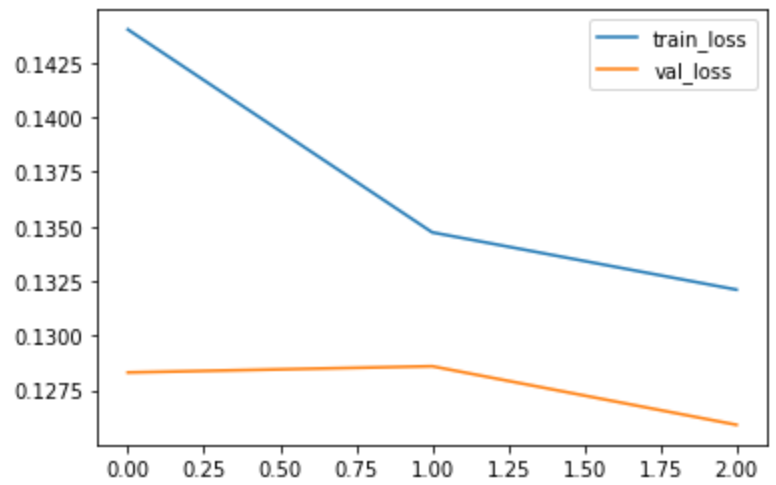
\includegraphics[width=0.45\textwidth]{../figures/deephit_losses_3_epoch.png}
\end{figure}

Метрики на ТОП 10\% оказались у DeepHit оказались хуже, чем у бейзлайновой CatBoost.

\begin{figure}[h!]
	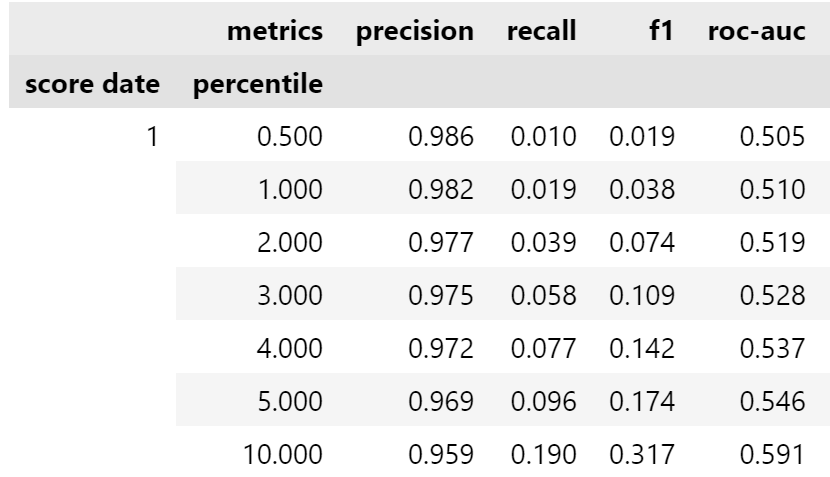
\includegraphics[width=0.45\textwidth]{../figures/deephit_reports_3_epoch.png}
	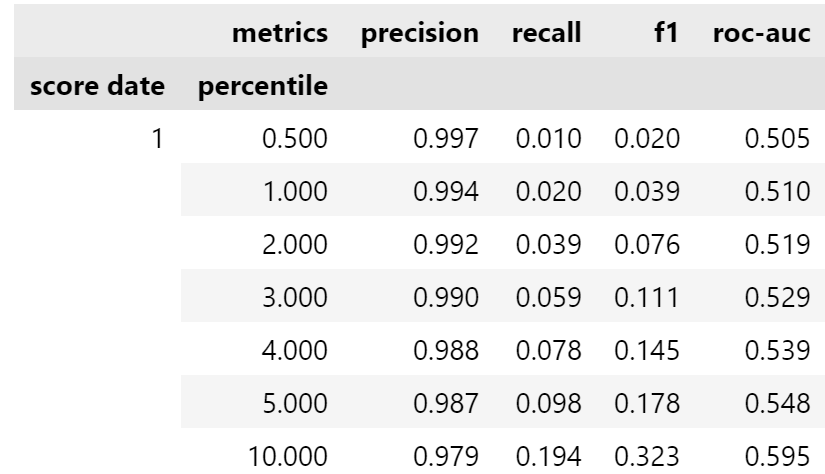
\includegraphics[width=0.45\textwidth]{../figures/catboost_reports.png}
\end{figure}

\subsubsection{Число эпох обучения = 50}

На этом этапе мы заметно увеличили число эпох обучения DeepHit. 

\bibliographystyle{unsrtnat}
\nocite{*}
\bibliography{references}


\end{document}